%!TEX root = main-doc.tex
%
% File: introduction.tex
%
% Date: ?
%
% Description:
%   Provides an introduction to the thesis and describes the
%   overall structure, chapter-by-chapter.
%
\chapter{Introduction}\label{chap:introduction}
\vspace{-1cm}
\summary{This chapter introduces the research and provides a detailed motivation for the significance of the research.}

%%%%%%%%%%%%%%%%%%%%%%%%%%%%%%%%%%%%%%%%%%%%%%%%%%%%%%%%%%%%%%%%%%%%%%%%%%%%%%%
\section{Problem Motivation}
Over recent years with the increase in smart-phone use, internet use, and virtually every activity leaving a digital trace, society has been able to store and collect more data, leading to the emergence of huge databases with quintillion bytes of data being produced everyday \cite{economist:2017:twm}. Data has been dubbed ``The world's most valuable resource'' in 2017 as economists believe it is ``the oil of the digital era'' with the five most valuable listed firms in the world for 2017 being data titans\cite{economist:2017:twm}. 

By combining different data sets, useful information can be retrieved from the stored data. Information resources are incredibly important and valuable in business management and decision-making \cite{golfarelli:2009:dwd,wang:2014sar}. By collecting lots of data, companies are able to improve their products and entice more clients with these improvements \cite{economist:2017:twm}. Due to their significance, these data assets must be stored properly and accessed easily \cite{golfarelli:2009:dwd}. Traditional data analysis tools are not able to handle such growing quantities of data. Thus various applications and technologies for managing big-data and high volume data-streams in data intensive computing is becoming essential. Further big-data, data-mining and machine learning are now of major concern in several scientific domains. Thus the field of “Big Data” research has materialised from the need to store such large quantities of information. Data analysis in all societal domains involves the storage, retrieval, processing and visualisation of huge databases \cite{otoo:2006:esa}. 

Big data is a rapidly growing on a global scale. However there is a bottleneck of technology that is required to extend the capabilities of the field. Several big data technologies are required that currently don't exist, including: architectures, algorithms, and techniques \cite{twala:2017:bda,moukhi:2015:dws}.

%%%%%%%%%%%%%%%%%%%%%%%%%%%%%%%%%%%%%%%%%%%%%%%%%%%%%%%%%%%%%%%%%%%%%%%%%%%%%%%
\section{Significance}
A new phenomenon, known as data warehousing, was developed as a result of the large quantities of data that need to be stored in recent years \cite{golfarelli:2009:dwd}. Data warehousing is a method used to combine multiple varied datasets into one complete and easily manipulated database as a decision support system. On-Line Analytical Processing (OLAP) can then be performed on these databases by an organisation in order to analyse the data, complete data-mining and determine trends. The organisation is then able to build business intelligent decisions by utilising the analysed data. Data warehousing has many applications in medical informatics and public-health, smart cities, mining, energy, physics and financial systems to name a few.

The storage of the datasets influences the accuracy, speed and performance of the data analysis and thus it is crucial to assess how this information is stored and accessed. Research over several years has concluded that multidimensional representation of data in data warehousing not only gives a good visual perspective of the data to the user, but also provides a storage scheme for efficient processing. Several research advancements have been made in multidimensional arrays in order to ensure that the datasets are efficient and inexpensive. Multi-dimensional arrays when used for their selection, aggregation, summation and other range queries are processed more efficiently than their SQL counter part in huge database queries. Since data in a data warehouse grows dynamically the multidimensional representation should also be expanded dynamically. These multidimensional datasets are continuously increasing by appending new data to the dataset as new information is added \cite{otoo:2006:esa}.

Recent breakthroughs in extendible multidimensional arrays have led to a new area of study in data warehousing, which requires further research and development. Efficient dynamic storage schemes for storing dense, extendible, multidimensional arrays by chunks have been developed \cite{nimako:2012:ced,pedereira:2015:cas}. However in data warehousing the corresponding multidimensional arrays are predominantly sparse arrays. It is thus important to analyse extendible multidimensional sparse arrays. There have been a number of advances made in the performance and efficiency of storage schemes for representing multidimensional sparse arrays \cite{otoo:2016:msa,goil:bess,otoo:2014:nas}. However, currently no storage or mapping techniques allow for the extendibility of multidimensional sparse arrays \cite{nimako:2016:cea}. Being able to utilize efficient extendible multidimensional sparse arrays will extend the capabilities and domains for data warehousing, data-mining and big-data analysis.
%With computation and storage costs being the most expensive part of data warehousing and data-mining,  %fix last sentence .....  high efficient processing - minimal mannaer (storage)

%%%%%%%%%%%%%%%%%%%%%%%%%%%%%%%%%%%%%%%%%%%%%%%%%%%%%%%%%%%%%%%%%%%%%%%%%%%%%%%
\section{Problem Statement}
The question raised is whether multidimensional sparse arrays can be stored in such a way that new elements and hyper-plane dimensions can be added. The problem that we are focused on requires the use of new storage techniques to investigate the extendibility of multidimensional sparse arrays with regards to computer performance and storage efficiencies.

An illustrative example of where data warehousing is used is given in Table \ref{tab:example}. Here we will have a fact table displaying the number of items sold on a particular day. This can be further extended into a data repository consisting of items sold per day per store as a relational table. In order to analyse the data to improve a company's sales, they might want to know the number of items sold, or which item is sold more on which day. I.e more carrots are sold on Wednesdays. In order to summarise these values and find patterns in the data these fact tables are converted into multidimensional arrays as shown in Figure \ref{fig:exampleDataWarehousing}.  Using these arrays, drill-down (or roll-down) and roll-out queries can be conducted to summarize the number of sales per week.

\begin{table}[H]
	\caption{A Typical Data Warehousing Fact Table.\label{tab:example}}
	\begin{center}
		\begin{tabular}{p{26mm}cp{35mm}}
			\hline
			{\textbf{Item}} & {\textbf{Time}} & {\textbf{ Amount}}\\
			\hline
			Apple   & Monday & 12 \\
			Orange  & Monday & 10\\
			Carrot  & Monday & 9\\
			Banana  & Monday & 9\\
			Grapefruit & Monday & 10\\
			Apple   & Tuesday & 7 \\
			Orange  & Tuesday & 8 \\
			Banana	& Tuesday & 18 \\
			Apple   & Wednesday & 5 \\
			Banana  & Wednesday & 3\\
			Carrot  & Wednesday & 10\\
			\hline
		\end{tabular}
	\end{center}
\end{table}

 \begin{figure}[H]
	\centering
	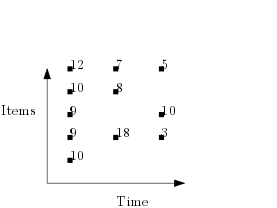
\includegraphics[width=0.6\linewidth]{exampleDataWarehouse}
	\caption{Fact Table Converted to a 2D Array}
	\label{fig:exampleDataWarehousing}
\end{figure}

%%%%%%%%%%%%%%%%%%%%%%%%%%%%%%%%%%%%%%%%%%%%%%%%%%%%%%%%%%%%%%%%%%%%%%%%%%%%%%%
\section{Application}
There are several problems that currently exist in the world that would utilize Big Data and data warehousing. A major example would be the frequency and quality of demographic statistics produced by countries as well as demographic statistics deficits. Such applications are particularly of major demand in developing countries.

\begin{itemize}
	\item There are 46 African countries operating without a complete birth and death registration system.
	\item Population censuses have not been conducted since 2010 in several African countries.
	\item Several African countries have not conducted an agricultural census in the last ten years. South Africa in particular held their last agricultural census in 2007.
\end{itemize}

Having up-to-date, reliable demographic statistics enables people within the population to partake in highly important activities. These include gaining quality education, formal employment, voting in elections, access to financial services, obtaining passports and obtaining IDs to name but a few. Reliable data also enables governments to budget better and improve the delivery of public goods and services \cite{mo:2015:sin}. A further application of data warehousing technologies used in the economic sector include tracking taxes, risk analysis and fraud detection. 

The field of application of data warehouse systems are also used in the trade sector to monitor inventory control, check up on customer care, and analyse company sales \cite{golfarelli:2009:dwd}.

%%%%%%%%%%%%%%%%%%%%%%%%%%%%%%%%%%%%%%%%%%%%%%%%%%%%%%%%%%%%%%%%%%%%%%%%%%%%%%%
\section{Early Results from Literature}
\textbf{NB - Still working on this section}

%%%%%%%%%%%%%%%%%%%%%%%%%%%%%%%%%%%%%%%%%%%%%%%%%%%%%%%%%%%%%%%%%%%%%%%%%%%%%%%
\section{Contribution to Field}
As data is constantly growing, there needs to be a method to provide for this extendibility. The aim of the proposed study is to improve the modelling and representation of extendible multidimensional sparse arrays so that useful compression and storage efficiency can be determined. The representation of the extendible multidimensional sparse arrays must include the characteristics of an array format, such that the array can take on any designed multiple hyper-plane dimensions. The characteristics of the array allow for easy data access. In addition, this allows for both drill-down and roll-out queries. Where drill-down queries allow for detailed data access and roll-out queries allow for summary data access.

The modelling of the extendible multidimensional sparse arrays will be able to contribute to developing algorithms that can process data at higher speeds, use less physical computational resources and improve the usage of computational power.

Our work addresses extendibility of the sparse array only, and does not concern the shrinking of the sparse array as data is never deleted from data warehouses \cite{golfarelli:2009:dwd}.

%%%%%%%%%%%%%%%%%%%%%%%%%%%%%%%%%%%%%%%%%%%%%%%%%%%%%%%%%%%%%%%%%%%%%%%%%%%%%%%
\section{Organisation of the Proposal}%%CHANGE TO DISSERTATION IN FUTURE
Chapter \ref{chap:background} provides a background on data warehousing and OLAP, extendible multidimensional dense arrays and multidimensional sparse arrays. Chapter \ref{chap:methodology} provides the proposed methodology for developing extendible multidimensional sparse array representations for data warehousing. The experimental set-up is provided in Chapter \ref{chap:experimentalsetup}. Chapter 5 details the preliminary results of the research. Expansion on the preliminary results is discussed in Chapter 6. Possible issues that could arise during the research as well as their proposed solutions are presented in Chapter 7. A schedule for the completion of the research is outlined in Chapter 8. A summary of the proposal is given in Chapter 9. 